\section{Durchführung}
\label{sec:Durchführung}
Der Versuchsaufbau ist in Abbildung \ref{fig:aufbau} zu sehen. Essentiel für den Aufbau sind Mikrofon und Lautsprecher, sowie verschiedene Resonatoren.
Die Messung und Auswertung erfolgt entweder über einen Sinusgenerator, welcher an den Lautsprecher angeschlossen ist.
Ein Oszilloskop wird über einen Frequenz-zu-Spannungs-Konverter, der in der Steuerelektronik verbaut ist, an das Mikrofon angeschlossen.
Die andere Auswertungsmethode wird mit einem Computer und dem Programm SpectrumSLC durchgeführt. Dazu werden Mikrofon und Lautsprecher direkt an den Computer angeschlossen.
\begin{figure}
    \centering
    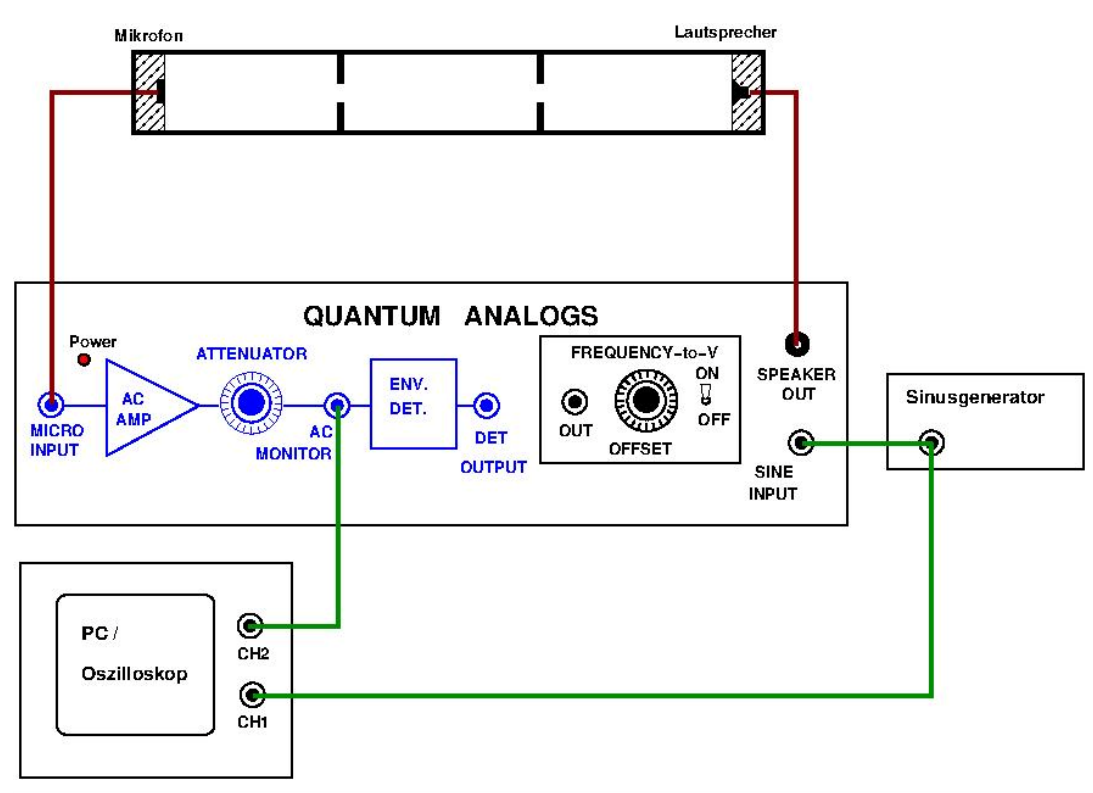
\includegraphics[width=\textwidth]{pictures/Aufbau.png}
    \caption{Prinzipieller Aufbau des Versuchs \cite{}}
    \label{fig:aufbau}
\end{figure}
\subsection{Vorbereitendes Experiment}
Im ersten Teil des Versuchs soll ein Frequenzspektrum von $\SI{0.1}{\kilo\hertz}$ bis $\SI{12}{\kilo\hertz}$ eines $\SI{50}{\milli\meter}$-Zylinders aufgenommen werden.
Das Mikrofon-Signal wird am 2-Kanal-Oszilloskop dargstellt, sowie an dem Computer abgespeichert.
Nach der Messung mit einem Zylinder wird ein weiterer hinzugefügt. Diese Schritte wiederholen sich bis zwölf Zylinder hintereinander gereiht sind.
Anschließend wird ein Frequenzspektrum eines $\SI{75}{\milli\meter}$-Zylinders aufgenommen.

\subsection{Wasserstoffatom}
Im folgenden Versuchsteil wird der Kugelresonator als klassisches Analogon zum Wasserstoffatom untersucht.
Der Kugelresonator besteht aus zwei Kugelhälften, wobei die untere mit Mikrofon und die obere mit einem Lautsprecher ausgestattet sind.
Beide sind $\ang{45;;}$ zur Horizontalen Ebene ausgerichtet.
Mit der Winkelskala am Außenrand der Halbkugeln lässt sich der Winkel $\alpha$ zwischen Lautsprecher und Mikrofon ablesen.
Am Anfang wird $\alpha = \ang{180;;}$ eingestellt.
\\
 Es folgt die Messung eines hochaufgelösten Frequenzspektrums von $\SI{0.1}{\kilo\hertz}$ bis $\SI{12}{\kilo\hertz}$ 
in $\SI{5}{\hertz}$-Schritten bei $\SI{60}{\milli\second}$ pro Schritt am Computer.
\\
Im nächsten Teil wird wieder das Oszilloskop angeschlossen und es werden die Frequenzen von $\SI{100}{\hertz}$ bis $\SI{10}{\kilo\hertz}$ durchlaufen.
Dabei werden von den Resonanzfrequenzen die Frequenz, Amplitude und Phasenverschiebung betrachten.
\\
Als nächstes werden am Computer hochaufgelöste Winkelabhängige Frequenzspektren aufgenommen. Diese werden in $\ang{5;;}$-Schritten von $0-\ang{180;;}$ bei gleichen Einstellungen wie zuvor aufgenommen.
Um die Kugelsymmetrie zu brechen wird im folgenden Teil ein $\SI{3}{\milli\meter}$ Zwischenring zwischen die Halbkugeln plaziert.
\\
Bei einem Winkel von $\ang{180;;}$ wird ein hochaufgelöstes Frequenzspektrum der Resonanzfrequenz bei $\SI{2.3}{\kilo\hertz}$ aufgenommen.
Dafür wird der Bereich $\SI{1.8}{\kilo\hertz}$ bis  $\SI{2.6}{\kilo\hertz}$ in  $\SI{1}{\hertz}$-Schritten bei gleicher Zeiteinstellung aufgenommen.
Dieser Versuchsteil wird erneut mit einem $\SI{6}{\milli\meter}$ Zwischenring und einer Kombination der beiden Ringe durchgeführt.

\subsection{Wasserstoffmolekül}
Zwischen die beiden Halbkugeln des Wasserstoff analogons werden zwei weitere Halbkugeln mit Loch eingesetzt, sodass zwei Kugelresonatoren mit einem offenem Verbindungsstück entstehen.
Die Halbkugeln werden so angeordet, dass das Mikrofon und der Lautsprecher bei einem Winkel von $\ang{180;;}$ liegen.
\\
Folgend wird ein hochaufgelöstes Frequenzspektrum, 
in dem Bereich von $\SI{2.2}{\kilo\hertz}$ bis $\SI{2.5}{\kilo\hertz}$ in  $\SI{1}{\hertz}$-Schritten mit $\SI{75}{\milli\second}$ pro Schritt, aufgenommen.
Dieser Versuchsteil wird mit Blenden mit $\SI{10}{\milli\meter}$, $\SI{13}{\milli\meter}$ und $\SI{16}{\milli\meter}$ Durchmesser erneut durchgeführt.
\\
Zuletzt wird ein Winkelaufgelöstes Spektrum mit einer $\SI{16}{\milli\meter}$ Blende aufgenommen. Der Messbereich und die Einstellungen sind dabei identisch zu den vorherigen Versuchsteil.
Die Messung erfolgt in $\ang{5;;}$-Schritten und geht von $\ang{0;;}$ bis $\ang{180;;}$. Des weiteren werden die Phasenverschiebungen der unteren und oberen Kugel bei den Resonanzfrequenzen aufgenommen.

\subsection{Eindimensionaler Festkörper}
Der letzte Versuchsteil wird aus einer Resonatorkette mit $\SI{16}{\milli\meter}$-Blenden aufgebaut.
Angefangen wird mit einer Blende zwischen zwei Resonatoren. Es wird ein Spektrum im Bereich von
$\SI{0.1}{\kilo\hertz}$ bis $\SI{12}{\kilo\hertz}$ in $\SI{5}{\hertz}$-Schritten mit $\SI{50}{\milli\second}$ pro Schritt aufgenommen.
Darauffolgend wird die Kette immer um einen Resonator mit Blende vergrößert bis 10 Resonatoren eingebaut sind. Pro hinzugefügtem Resonator wird ein Spektrum
wie oben beschrieben aufgenommen.
\\
Das Experiment wird mit 2,4 und zehn Resonatoren wiederholt, wobei einmal $\SI{10}{\milli\meter}$-Blenden und einmal $\SI{13}{\milli\meter}$-Blenden
verwendet werden.
\\
Als nächstes wird einer der zehn Zylinder durch einen $\SI{75}{\milli\meter}$, $\SI{37.5}{\milli\meter}$ und einen $\SI{62.5}{\milli\meter}$ Zylinder ersetzt und
es wird erneut ein Spektrum aufgenommen.
\\
Der nächste Versuchsteil wird mit zehn abwechselnd angeordneten Resonatoren mit $\SI{16}{\milli\meter}$-Blenden aufgebaut.
Es wird wieder ein Frequenzspektrum wie zuvor aufgenommen.
\\
Im letzten Versuchteil wird aus acht $\SI{50}{\milli\meter}$-Resonatoren mit abwechselnd $\SI{13}{\milli\meter}$ und $\SI{16}{\milli\meter}$-Blenden dazwischen
eine Resonatorkette aufgebaut und ein weiteres Spektrum entnommen.